%!TEX program = xelatex
%%%%%%%%%%%%%%%%%%%%%%%这是导言部分的开始%%%%%%%%

%========= 导言部分声明文档的类型=================
\documentclass{article}

	%=========导言部分可可以加载宏包=================
	\usepackage{amsmath}                % 数学公式排版宏包
	\usepackage{amssymb}                % 数学符号命令宏包
	\usepackage{amsthm}                 % 数学定理宏包
	\usepackage[UTF8]{ctex}             % 中文输入宏包
	\usepackage[a4paper]{geometry}      % 页面设置宏包
	\usepackage{setspace}               % 行间距宏包
	\usepackage{graphicx}               % 图片宏包
	\usepackage{listings}               % 代码宏包
	\usepackage{color}					% 颜色宏包
	\usepackage{xcolor}                 % 颜色处理宏包
	\usepackage{float}                  % 浮动对象式样宏包
	\usepackage{fontspec}
	\usepackage{enumerate}				% 列举编号包
	
	%=========页面设置==============================
	\geometry{left=1cm,right=1cm,top=1cm,bottom=2cm}
	\onehalfspacing
	\setlength\parindent{0em}

	%=========代码格式设置============================
	\definecolor{dkgreen}{rgb}{0,0.6,0}
	\definecolor{gray}{rgb}{0.5,0.5,0.5}
	\definecolor{mauve}{rgb}{0.58,0,0.82}
	% \setmonofont{Consolas}
	\lstset{
		numbers = left, 	
		numberstyle = \color{gray}, 
		keywordstyle = \color{blue},
		commentstyle = \color{dkgreen}, 
		stringstyle = \color{mauve},
		basicstyle = \ttfamily,
		breaklines = true,
		frame = shadowbox, % 阴影效果
		rulesepcolor = \color{ red!20!green!20!blue!20} ,
		escapeinside = ``, % 英文分号中可写入中文
		xleftmargin = 2em,xrightmargin=2em, aboveskip=1em,
		framexleftmargin = 2em
	} 

%=========导言部分可以定义标题信息===============
\title{组会报告}
\author{徐益}
\date{\today}
%%%%%%%%%%%%%%%%%%%%%%%这是导言部分的结束%%%%%%%%%

%%%%%%%%%%%%%%%%%%%%%%%这是正文部分的开始%%%%%%%%%
\begin{document}

%=========生成标题================================
\maketitle

%=========开始正文的输入==========================

%===========第一节=================
\section{工作内容}
1. 各译码算法的C语言实现

2. 实现LDPC编译码的mex函数编写

3. 测试LDPC速率匹配模块

%===========第一节=================
\section{译码算法C语言实现中的数据结构选择}
\subsection{稀疏矩阵结构}
\lstset{language=C++}
\begin{lstlisting}
typedef struct		/* Representation of a sparse matrix */
{ 
  int n_rows;		  /* Number of rows in the matrix */
  int n_cols;		  /* Number of columns in the matrix */

  mod2entry *rows;	  /* Pointer to array of row headers */
  mod2entry *cols;	  /* Pointer to array of column headers */

  mod2block *blocks;	  /* Blocks that have been allocated */
  mod2entry *next_free;	  /* Next free entry */

} mod2sparse;
\end{lstlisting}
\subsection{变量-校验节点结构}
\lstset{language=C++}
\begin{lstlisting}
typedef struct variable_node
{
	int8_t degree;	// number of connective check nodes
	int16_t *index;	// index of connective check nodes
	float* message;	// message from vn to cn
	int8_t pointer;	// pointer to the message that will be used
	float judge_message;
} variable_node;

typedef struct check_node
{
	int8_t degree;	// number of connective variable nodes
	int16_t *index;	// index of connective variable nodes
	float* message;	// message from cn to vn
	int8_t pointer;	// pointer to the message that will be used
} check_node;
\end{lstlisting}

%===========第二节=================
\section{实现LDPC编译码的mex函数编写}
\subsection{常见问题}
\begin{figure}[H]
	\centering
	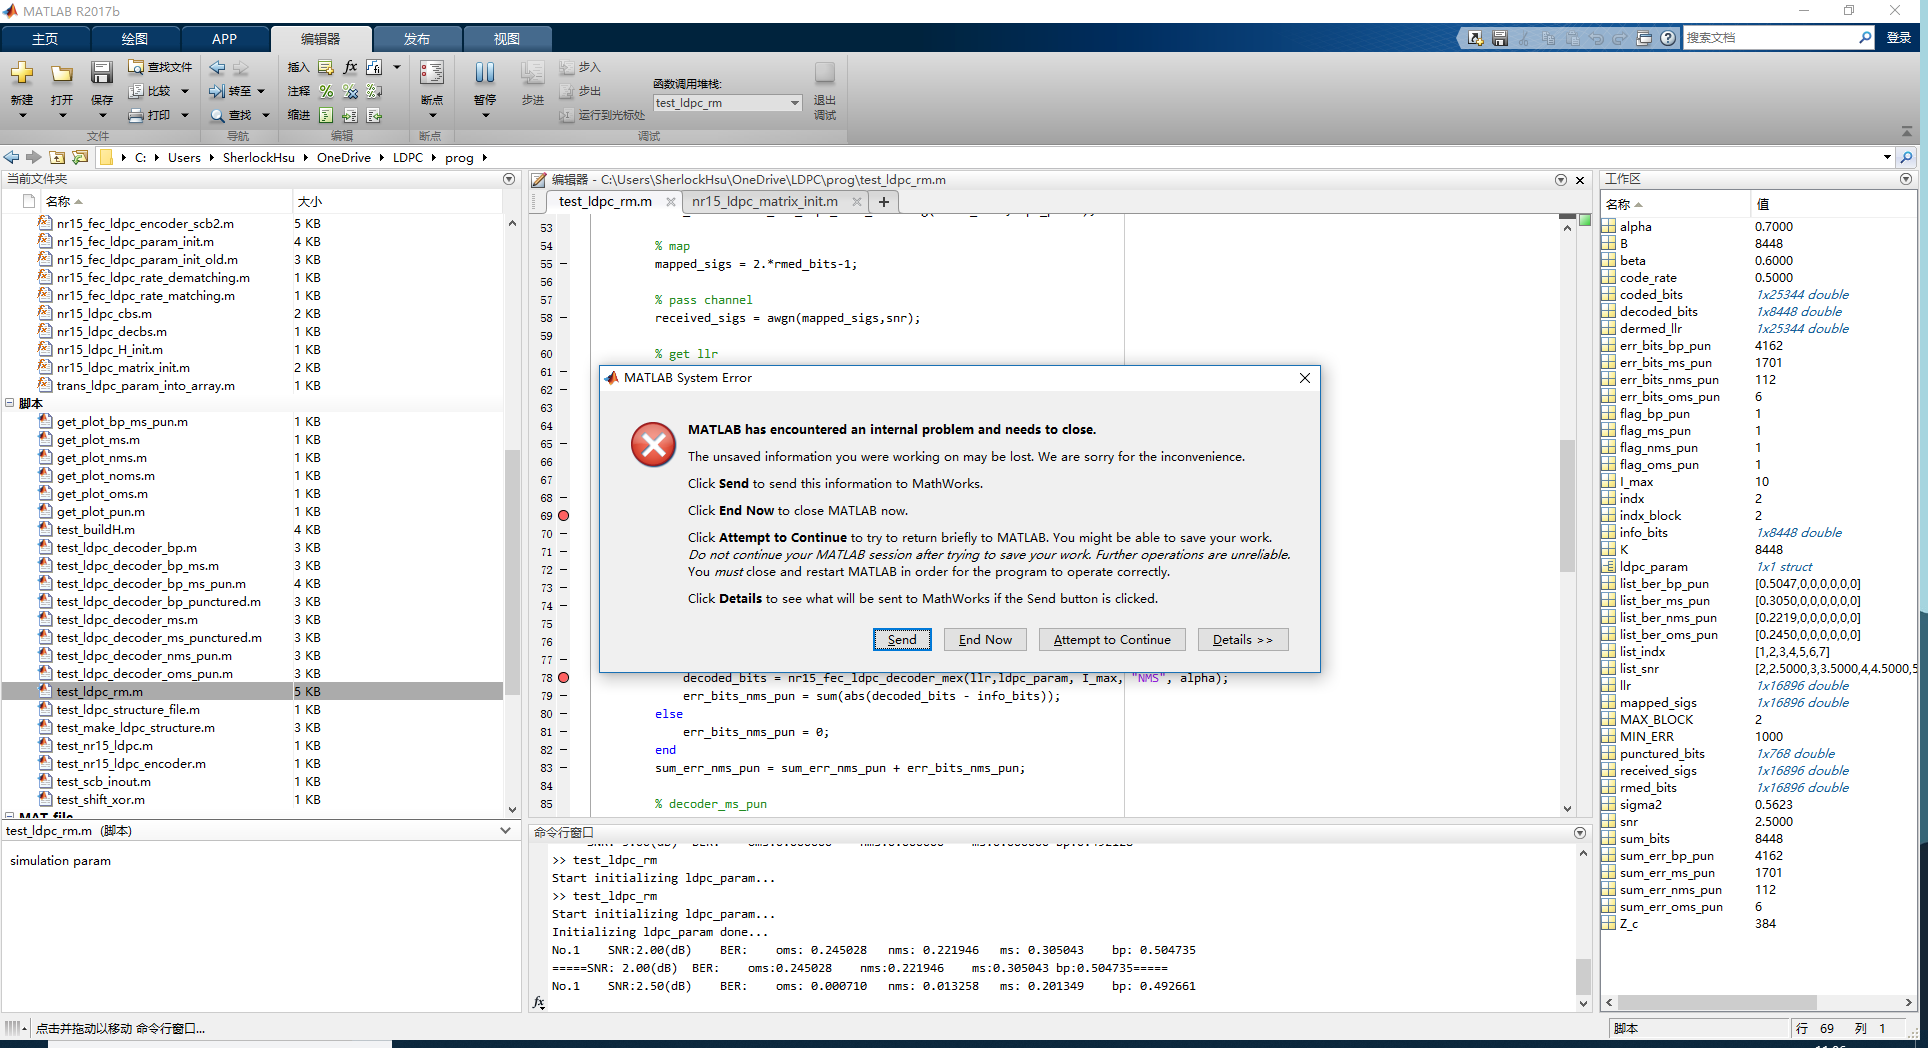
\includegraphics[width = \textwidth]{err.png}
	\caption{mex函数运行失败}
\end{figure}
\subsection{常见原因}
1. 缺少头文件。由于VS会自动引入部分头文件,部分头文件缺少较难察觉,如stdlib.h。\\
2. 内存泄漏。部分结构体内指向的空间未即使释放,长时间运行会导致程序崩溃。\\
3. 内存释放错误。错误将mex接口函数的输入指针指向的空间释放。\\
\subsubsection{吞吐量测试}
\begin{table}[H]
	\caption{不同译码算法的吞吐量($N=25344,R=0.5,I_{max}=100$)}
	\centering
	\begin{tabular}{|l|l|l|l|}% 通过添加 | 来表示是否需要绘制竖线
		\hline  % 在表格最上方绘制横线
		SNR   & MS         & NMS        & OMS        \\
		\hline
		1.5dB & 51.858kbps & 43.754kbps & 96.914kbps \\
		\hline
		3.0dB & 153.12kbps & 161.00kbps & 173.11kbps \\
		\hline  % 在表格最下方绘制横线
	\end{tabular}
\end{table}

%===========第三节=================
\section{测试LDPC速率匹配模块}
\begin{figure}[H]
	\centering
	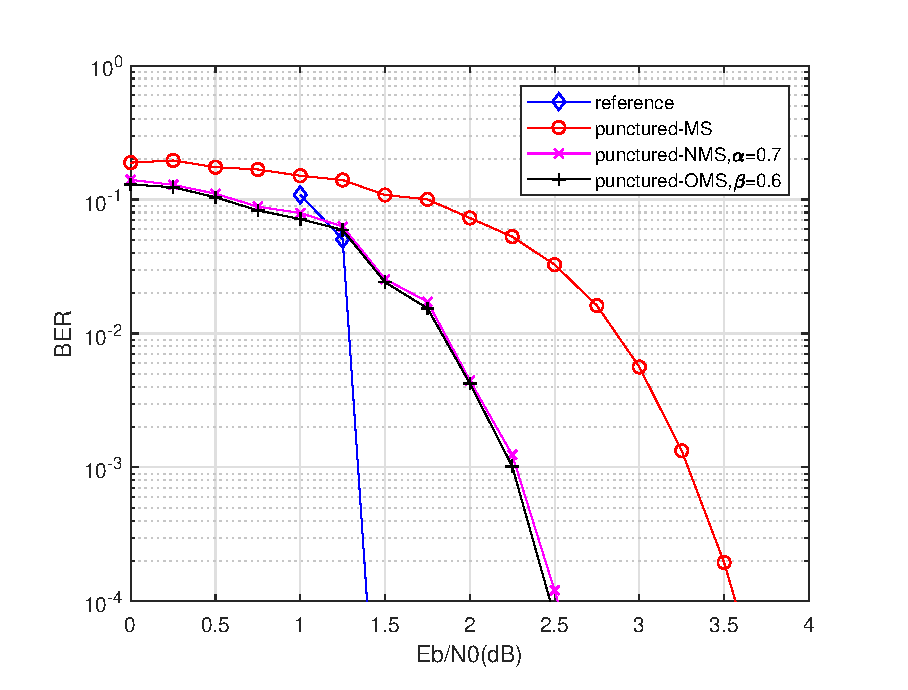
\includegraphics[width = .75\textwidth]{noms_r12_Imax10.eps}
	\caption{{不同译码算法的误码性能与参考值对比($N=25344,R=0.5,I_{max}=10$)}}
\end{figure}
\begin{figure}[H]
	\centering
	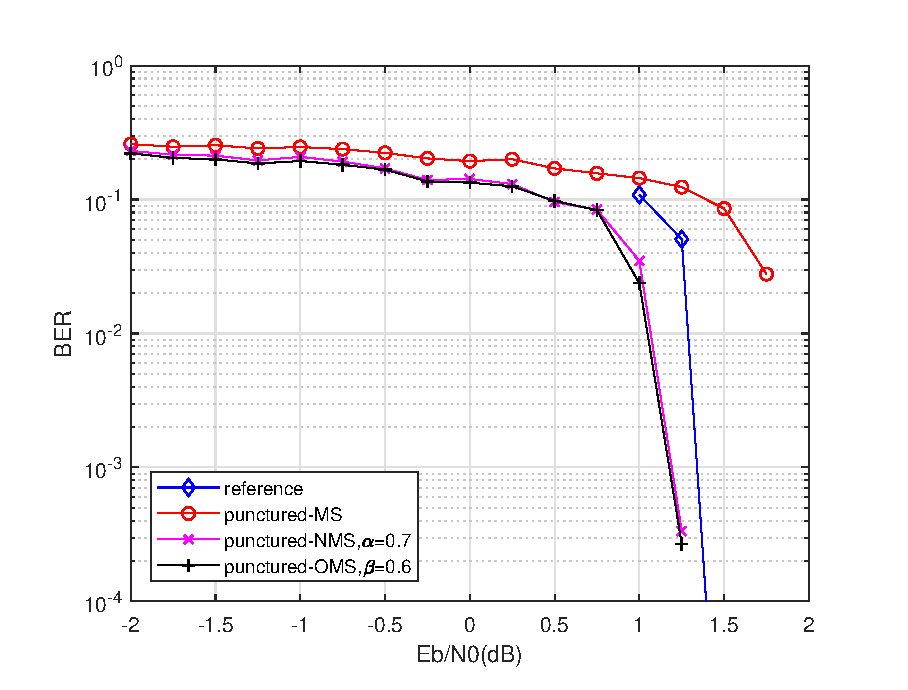
\includegraphics[width = .75\textwidth]{noms_r12.eps}
	\caption{{不同译码算法的误码性能与参考值对比($N=25344,R=0.5,I_{max}=100$)}}
\end{figure}
\begin{figure}[H]
	\centering
	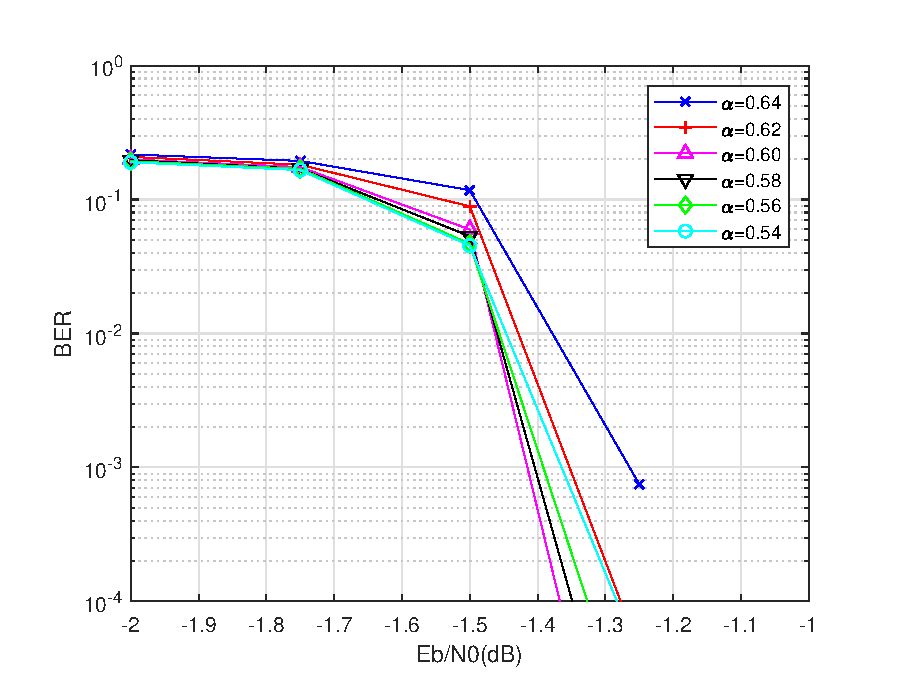
\includegraphics[width = .75\textwidth]{nms064054.eps}
	\caption{{不同$\alpha$的NMS算法误码性能($N=25344,R=0.5,I_{max}=100$)}}
\end{figure}
\begin{figure}[H]
	\centering
	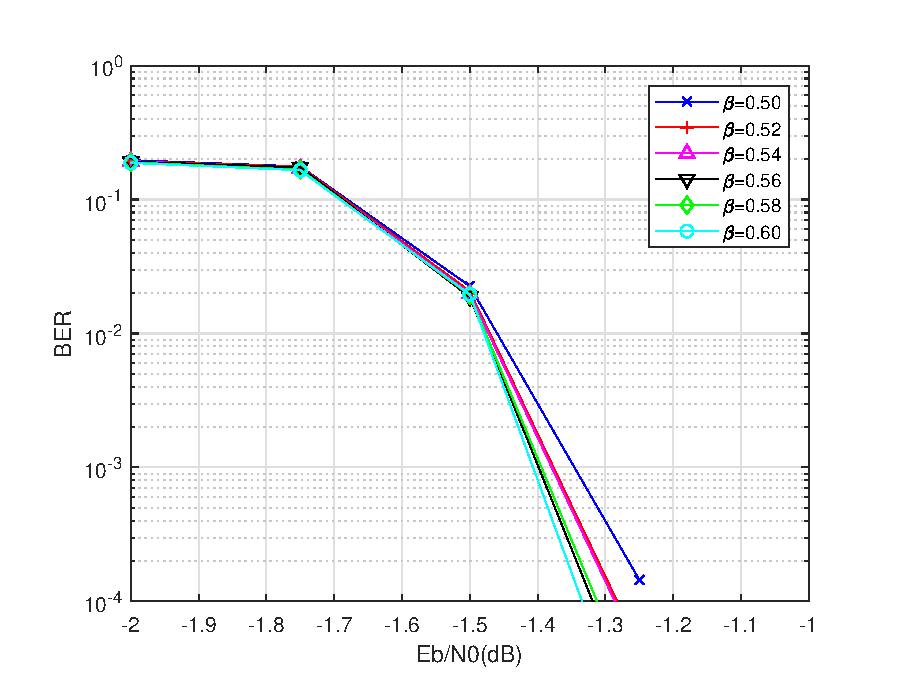
\includegraphics[width = .75\textwidth]{oms0506.eps}
	\caption{{不同$\beta$的OMS算法误码性能($N=25344,R=0.5,I_{max}=100$)}}
\end{figure}

%===========第四节=================
\section{仍存在问题}
\begin{figure}[H]
	\centering
	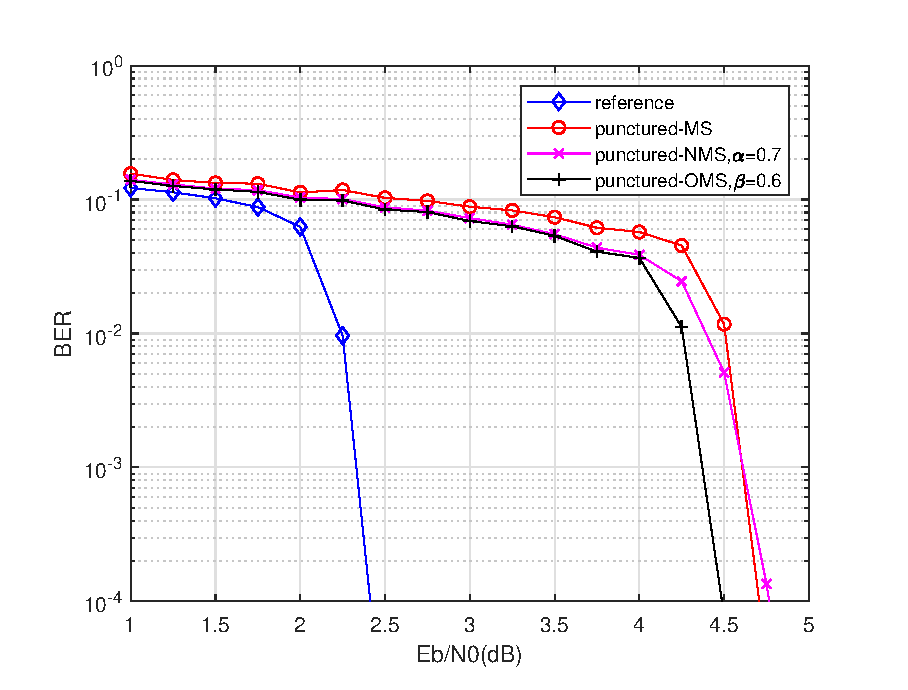
\includegraphics[width = .75\textwidth]{noms_r34.eps}
	\caption{{不同译码算法的误码性能与参考值对比($N=25344,R=0.75,I_{max}=100$)}}
\end{figure}

%===========下周计划=================
% \section{下阶段计划}
% 实现LDPC剩余的mex函数

\end{document}
%%%%%%%%%%%%%%%%%%%%%%%这是正文部分的结束%%%%%%%%%%%%